% Options for packages loaded elsewhere
\PassOptionsToPackage{unicode}{hyperref}
\PassOptionsToPackage{hyphens}{url}
%
\documentclass[
]{article}
\title{Capitulo 2: Introduccion a la Estadistica Inferencial}
\author{Dereck Amesquita}
\date{6/4/2021}

\usepackage{amsmath,amssymb}
\usepackage{lmodern}
\usepackage{iftex}
\ifPDFTeX
  \usepackage[T1]{fontenc}
  \usepackage[utf8]{inputenc}
  \usepackage{textcomp} % provide euro and other symbols
\else % if luatex or xetex
  \usepackage{unicode-math}
  \defaultfontfeatures{Scale=MatchLowercase}
  \defaultfontfeatures[\rmfamily]{Ligatures=TeX,Scale=1}
\fi
% Use upquote if available, for straight quotes in verbatim environments
\IfFileExists{upquote.sty}{\usepackage{upquote}}{}
\IfFileExists{microtype.sty}{% use microtype if available
  \usepackage[]{microtype}
  \UseMicrotypeSet[protrusion]{basicmath} % disable protrusion for tt fonts
}{}
\makeatletter
\@ifundefined{KOMAClassName}{% if non-KOMA class
  \IfFileExists{parskip.sty}{%
    \usepackage{parskip}
  }{% else
    \setlength{\parindent}{0pt}
    \setlength{\parskip}{6pt plus 2pt minus 1pt}}
}{% if KOMA class
  \KOMAoptions{parskip=half}}
\makeatother
\usepackage{xcolor}
\IfFileExists{xurl.sty}{\usepackage{xurl}}{} % add URL line breaks if available
\IfFileExists{bookmark.sty}{\usepackage{bookmark}}{\usepackage{hyperref}}
\hypersetup{
  pdftitle={Capitulo 2: Introduccion a la Estadistica Inferencial},
  pdfauthor={Dereck Amesquita},
  hidelinks,
  pdfcreator={LaTeX via pandoc}}
\urlstyle{same} % disable monospaced font for URLs
\usepackage[margin=1in]{geometry}
\usepackage{color}
\usepackage{fancyvrb}
\newcommand{\VerbBar}{|}
\newcommand{\VERB}{\Verb[commandchars=\\\{\}]}
\DefineVerbatimEnvironment{Highlighting}{Verbatim}{commandchars=\\\{\}}
% Add ',fontsize=\small' for more characters per line
\usepackage{framed}
\definecolor{shadecolor}{RGB}{248,248,248}
\newenvironment{Shaded}{\begin{snugshade}}{\end{snugshade}}
\newcommand{\AlertTok}[1]{\textcolor[rgb]{0.94,0.16,0.16}{#1}}
\newcommand{\AnnotationTok}[1]{\textcolor[rgb]{0.56,0.35,0.01}{\textbf{\textit{#1}}}}
\newcommand{\AttributeTok}[1]{\textcolor[rgb]{0.77,0.63,0.00}{#1}}
\newcommand{\BaseNTok}[1]{\textcolor[rgb]{0.00,0.00,0.81}{#1}}
\newcommand{\BuiltInTok}[1]{#1}
\newcommand{\CharTok}[1]{\textcolor[rgb]{0.31,0.60,0.02}{#1}}
\newcommand{\CommentTok}[1]{\textcolor[rgb]{0.56,0.35,0.01}{\textit{#1}}}
\newcommand{\CommentVarTok}[1]{\textcolor[rgb]{0.56,0.35,0.01}{\textbf{\textit{#1}}}}
\newcommand{\ConstantTok}[1]{\textcolor[rgb]{0.00,0.00,0.00}{#1}}
\newcommand{\ControlFlowTok}[1]{\textcolor[rgb]{0.13,0.29,0.53}{\textbf{#1}}}
\newcommand{\DataTypeTok}[1]{\textcolor[rgb]{0.13,0.29,0.53}{#1}}
\newcommand{\DecValTok}[1]{\textcolor[rgb]{0.00,0.00,0.81}{#1}}
\newcommand{\DocumentationTok}[1]{\textcolor[rgb]{0.56,0.35,0.01}{\textbf{\textit{#1}}}}
\newcommand{\ErrorTok}[1]{\textcolor[rgb]{0.64,0.00,0.00}{\textbf{#1}}}
\newcommand{\ExtensionTok}[1]{#1}
\newcommand{\FloatTok}[1]{\textcolor[rgb]{0.00,0.00,0.81}{#1}}
\newcommand{\FunctionTok}[1]{\textcolor[rgb]{0.00,0.00,0.00}{#1}}
\newcommand{\ImportTok}[1]{#1}
\newcommand{\InformationTok}[1]{\textcolor[rgb]{0.56,0.35,0.01}{\textbf{\textit{#1}}}}
\newcommand{\KeywordTok}[1]{\textcolor[rgb]{0.13,0.29,0.53}{\textbf{#1}}}
\newcommand{\NormalTok}[1]{#1}
\newcommand{\OperatorTok}[1]{\textcolor[rgb]{0.81,0.36,0.00}{\textbf{#1}}}
\newcommand{\OtherTok}[1]{\textcolor[rgb]{0.56,0.35,0.01}{#1}}
\newcommand{\PreprocessorTok}[1]{\textcolor[rgb]{0.56,0.35,0.01}{\textit{#1}}}
\newcommand{\RegionMarkerTok}[1]{#1}
\newcommand{\SpecialCharTok}[1]{\textcolor[rgb]{0.00,0.00,0.00}{#1}}
\newcommand{\SpecialStringTok}[1]{\textcolor[rgb]{0.31,0.60,0.02}{#1}}
\newcommand{\StringTok}[1]{\textcolor[rgb]{0.31,0.60,0.02}{#1}}
\newcommand{\VariableTok}[1]{\textcolor[rgb]{0.00,0.00,0.00}{#1}}
\newcommand{\VerbatimStringTok}[1]{\textcolor[rgb]{0.31,0.60,0.02}{#1}}
\newcommand{\WarningTok}[1]{\textcolor[rgb]{0.56,0.35,0.01}{\textbf{\textit{#1}}}}
\usepackage{graphicx}
\makeatletter
\def\maxwidth{\ifdim\Gin@nat@width>\linewidth\linewidth\else\Gin@nat@width\fi}
\def\maxheight{\ifdim\Gin@nat@height>\textheight\textheight\else\Gin@nat@height\fi}
\makeatother
% Scale images if necessary, so that they will not overflow the page
% margins by default, and it is still possible to overwrite the defaults
% using explicit options in \includegraphics[width, height, ...]{}
\setkeys{Gin}{width=\maxwidth,height=\maxheight,keepaspectratio}
% Set default figure placement to htbp
\makeatletter
\def\fps@figure{htbp}
\makeatother
\setlength{\emergencystretch}{3em} % prevent overfull lines
\providecommand{\tightlist}{%
  \setlength{\itemsep}{0pt}\setlength{\parskip}{0pt}}
\setcounter{secnumdepth}{-\maxdimen} % remove section numbering
\ifLuaTeX
  \usepackage{selnolig}  % disable illegal ligatures
\fi

\begin{document}
\maketitle

\hypertarget{la-regresiuxf3n-lineal}{%
\section{La regresión Lineal}\label{la-regresiuxf3n-lineal}}

Podemos medir el efecto lineal que tiene una variable sobre otra con la
regresión lineal. \[y = a+bx\] En el capitulo de estadística inferencial
se abordaran los mínimos cuadrados ordinarios que nos ayudaran a obtener
el valor de b.

\begin{Shaded}
\begin{Highlighting}[]
\NormalTok{data}\OtherTok{=}\StringTok{"https://raw.githubusercontent.com/dereckamesquita/Learning{-}Before{-}Estadistica/main/datasets/bodyfat.txt"}
\NormalTok{datos}\OtherTok{=}\FunctionTok{read.table}\NormalTok{(data, }\AttributeTok{header =} \ConstantTok{TRUE}\NormalTok{)}
\NormalTok{datosn}\OtherTok{=}\NormalTok{datos[,}\FunctionTok{c}\NormalTok{(}\DecValTok{2}\NormalTok{,}\DecValTok{4}\NormalTok{)]}
\FunctionTok{names}\NormalTok{(datosn)}\OtherTok{=}\FunctionTok{c}\NormalTok{(}\StringTok{"Grasa"}\NormalTok{,}\StringTok{"Peso"}\NormalTok{)}
\FunctionTok{str}\NormalTok{(datosn)}
\end{Highlighting}
\end{Shaded}

\begin{verbatim}
## 'data.frame':    252 obs. of  2 variables:
##  $ Grasa: num  12.3 6.1 25.3 10.4 28.7 20.9 19.2 12.4 4.1 11.7 ...
##  $ Peso : num  154 173 154 185 184 ...
\end{verbatim}

\begin{Shaded}
\begin{Highlighting}[]
\CommentTok{\# Regresion}
\CommentTok{\#lm(y\textasciitilde{}x) \#Esto se lee como formula es decir: Y de X o y=ƒ(X) }
\CommentTok{\#Alt+159 = ƒ}
\NormalTok{regre1}\OtherTok{=}\FunctionTok{lm}\NormalTok{(Peso}\SpecialCharTok{\textasciitilde{}}\NormalTok{Grasa, }\AttributeTok{data=}\NormalTok{datosn)}
\FunctionTok{lm}\NormalTok{(datosn}\SpecialCharTok{$}\NormalTok{Peso}\SpecialCharTok{\textasciitilde{}}\NormalTok{datosn}\SpecialCharTok{$}\NormalTok{Grasa)}
\end{Highlighting}
\end{Shaded}

\begin{verbatim}
## 
## Call:
## lm(formula = datosn$Peso ~ datosn$Grasa)
## 
## Coefficients:
##  (Intercept)  datosn$Grasa  
##      137.738         2.151
\end{verbatim}

\hypertarget{graficando-la-regresion-lineal}{%
\subsection{Graficando la regresion
lineal}\label{graficando-la-regresion-lineal}}

\begin{Shaded}
\begin{Highlighting}[]
\FunctionTok{plot}\NormalTok{(datosn)}
\FunctionTok{abline}\NormalTok{(regre1, }\AttributeTok{col=}\StringTok{"blue"}\NormalTok{)}
\end{Highlighting}
\end{Shaded}

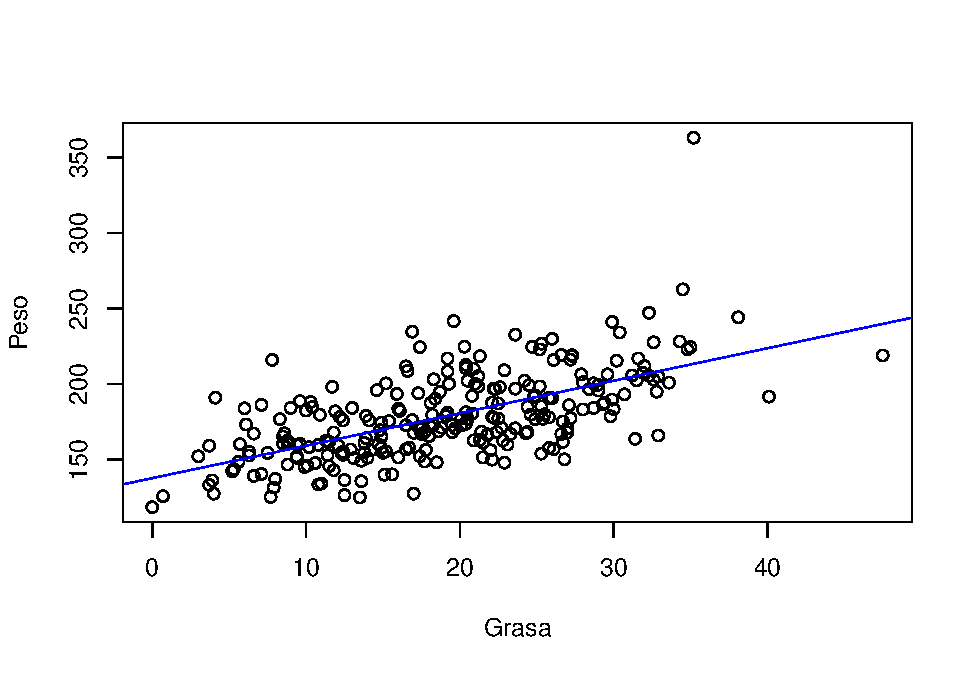
\includegraphics{Teoria4_files/figure-latex/Grafico-1.pdf}

\hypertarget{el-coeficiente-de-determinacion-r2}{%
\subsection{El coeficiente de determinacion
R2}\label{el-coeficiente-de-determinacion-r2}}

\begin{Shaded}
\begin{Highlighting}[]
\FunctionTok{summary}\NormalTok{(regre1) }\CommentTok{\# Nos arroja la inform acion mas importante de nuestra regresion}
\end{Highlighting}
\end{Shaded}

\begin{verbatim}
## 
## Call:
## lm(formula = Peso ~ Grasa, data = datosn)
## 
## Residuals:
##     Min      1Q  Median      3Q     Max 
## -46.799 -14.999  -3.469  11.860 149.709 
## 
## Coefficients:
##             Estimate Std. Error t value Pr(>|t|)    
## (Intercept) 137.7375     3.6684   37.55   <2e-16 ***
## Grasa         2.1507     0.1756   12.25   <2e-16 ***
## ---
## Signif. codes:  0 '***' 0.001 '**' 0.01 '*' 0.05 '.' 0.1 ' ' 1
## 
## Residual standard error: 23.28 on 250 degrees of freedom
## Multiple R-squared:  0.3751, Adjusted R-squared:  0.3726 
## F-statistic:   150 on 1 and 250 DF,  p-value: < 2.2e-16
\end{verbatim}

\begin{Shaded}
\begin{Highlighting}[]
\FunctionTok{summary}\NormalTok{(regre1)}\SpecialCharTok{$}\NormalTok{r.squared }\CommentTok{\#Nos arroja solo el R2}
\end{Highlighting}
\end{Shaded}

\begin{verbatim}
## [1] 0.3750509
\end{verbatim}

\hypertarget{escalas-logaritmicas}{%
\subsection{Escalas Logaritmicas}\label{escalas-logaritmicas}}

\begin{Shaded}
\begin{Highlighting}[]
\NormalTok{dep}\OtherTok{=}\FunctionTok{c}\NormalTok{(}\FloatTok{1.2}\NormalTok{,}\FloatTok{3.6}\NormalTok{,}\DecValTok{12}\NormalTok{,}\DecValTok{36}\NormalTok{)}
\NormalTok{ind}\OtherTok{=}\FunctionTok{c}\NormalTok{(}\DecValTok{20}\NormalTok{,}\DecValTok{35}\NormalTok{,}\DecValTok{61}\NormalTok{,}\DecValTok{82}\NormalTok{)}
\CommentTok{\#Graficos}
\FunctionTok{par}\NormalTok{(}\AttributeTok{mfrow =} \FunctionTok{c}\NormalTok{(}\DecValTok{1}\NormalTok{, }\DecValTok{2}\NormalTok{))}\CommentTok{\#Juntar dos plots}
\FunctionTok{plot}\NormalTok{(ind,dep, }\AttributeTok{main =} \StringTok{"Escala lineal"}\NormalTok{)}
\FunctionTok{plot}\NormalTok{(ind,dep, }\AttributeTok{log=}\StringTok{"y"}\NormalTok{, }\AttributeTok{main =} \StringTok{"Escala Logaritmica"}\NormalTok{)}
\end{Highlighting}
\end{Shaded}

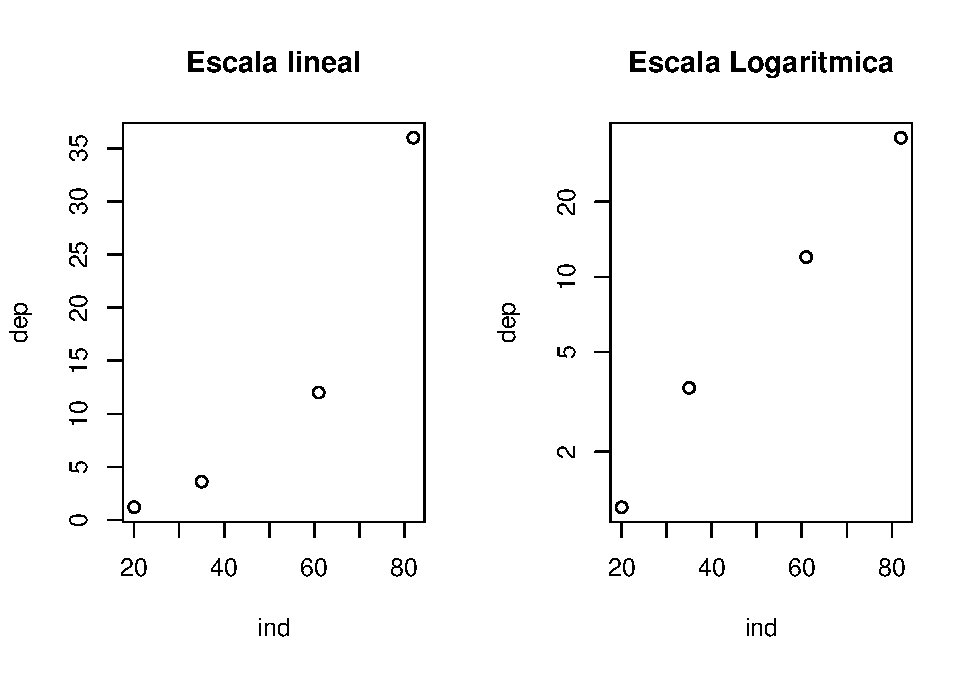
\includegraphics{Teoria4_files/figure-latex/Graficos en dos escalas-1.pdf}

\begin{Shaded}
\begin{Highlighting}[]
\NormalTok{regrelognivel}\OtherTok{=}\FunctionTok{lm}\NormalTok{(}\FunctionTok{log10}\NormalTok{(dep)}\SpecialCharTok{\textasciitilde{}}\NormalTok{ind)}
\FunctionTok{summary}\NormalTok{(regrelognivel)}
\end{Highlighting}
\end{Shaded}

\begin{verbatim}
## 
## Call:
## lm(formula = log10(dep) ~ ind)
## 
## Residuals:
##         1         2         3         4 
## -0.054845  0.074624 -0.005094 -0.014686 
## 
## Coefficients:
##              Estimate Std. Error t value Pr(>|t|)   
## (Intercept) -0.329510   0.076575  -4.303   0.0500 * 
## ind          0.023177   0.001394  16.626   0.0036 **
## ---
## Signif. codes:  0 '***' 0.001 '**' 0.01 '*' 0.05 '.' 0.1 ' ' 1
## 
## Residual standard error: 0.0664 on 2 degrees of freedom
## Multiple R-squared:  0.9928, Adjusted R-squared:  0.9892 
## F-statistic: 276.4 on 1 and 2 DF,  p-value: 0.003598
\end{verbatim}

\begin{Shaded}
\begin{Highlighting}[]
\CommentTok{\#Grafico}
\FunctionTok{plot}\NormalTok{(ind,dep,}\AttributeTok{main=}\StringTok{"Curva de regresion"}\NormalTok{)}
\FunctionTok{curve}\NormalTok{(}\FloatTok{1.054}\SpecialCharTok{\^{}}\NormalTok{x}\SpecialCharTok{*}\FloatTok{0.468}\NormalTok{, }\AttributeTok{add=}\ConstantTok{TRUE}\NormalTok{, }\AttributeTok{col=}\StringTok{"lightblue"}\NormalTok{)}
\end{Highlighting}
\end{Shaded}

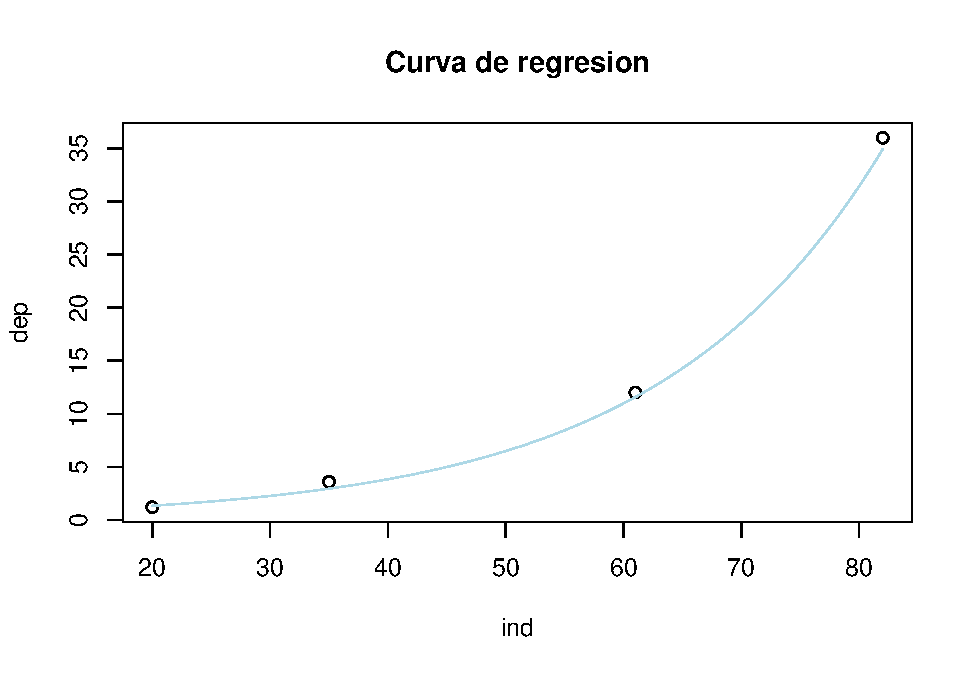
\includegraphics{Teoria4_files/figure-latex/Regresion exponencial-1.pdf}

\hypertarget{regresiones-potenciales}{%
\subsection{Regresiones potenciales}\label{regresiones-potenciales}}

\begin{Shaded}
\begin{Highlighting}[]
\NormalTok{tiempo }\OtherTok{=} \DecValTok{1}\SpecialCharTok{:}\DecValTok{10}
\NormalTok{gramos }\OtherTok{=} \FunctionTok{c}\NormalTok{(}\FloatTok{0.097}\NormalTok{,}\FloatTok{0.709}\NormalTok{,}\FloatTok{2.698}\NormalTok{,}\FloatTok{6.928}\NormalTok{,}\FloatTok{15.242}\NormalTok{,}\FloatTok{29.944}\NormalTok{,}\FloatTok{52.902}\NormalTok{,}\FloatTok{83.903}\NormalTok{,}\FloatTok{120.612}\NormalTok{,}\FloatTok{161.711}\NormalTok{)}
\NormalTok{d.f }\OtherTok{=} \FunctionTok{data.frame}\NormalTok{(tiempo,gramos)}
\CommentTok{\# Graficas}
\FunctionTok{par}\NormalTok{(}\AttributeTok{mfrow=} \FunctionTok{c}\NormalTok{(}\DecValTok{1}\NormalTok{,}\DecValTok{3}\NormalTok{))}
\FunctionTok{plot}\NormalTok{(d.f)}
\FunctionTok{plot}\NormalTok{(d.f, }\AttributeTok{log=}\StringTok{"y"}\NormalTok{)}
\FunctionTok{plot}\NormalTok{(d.f, }\AttributeTok{log=}\StringTok{"xy"}\NormalTok{)}
\end{Highlighting}
\end{Shaded}

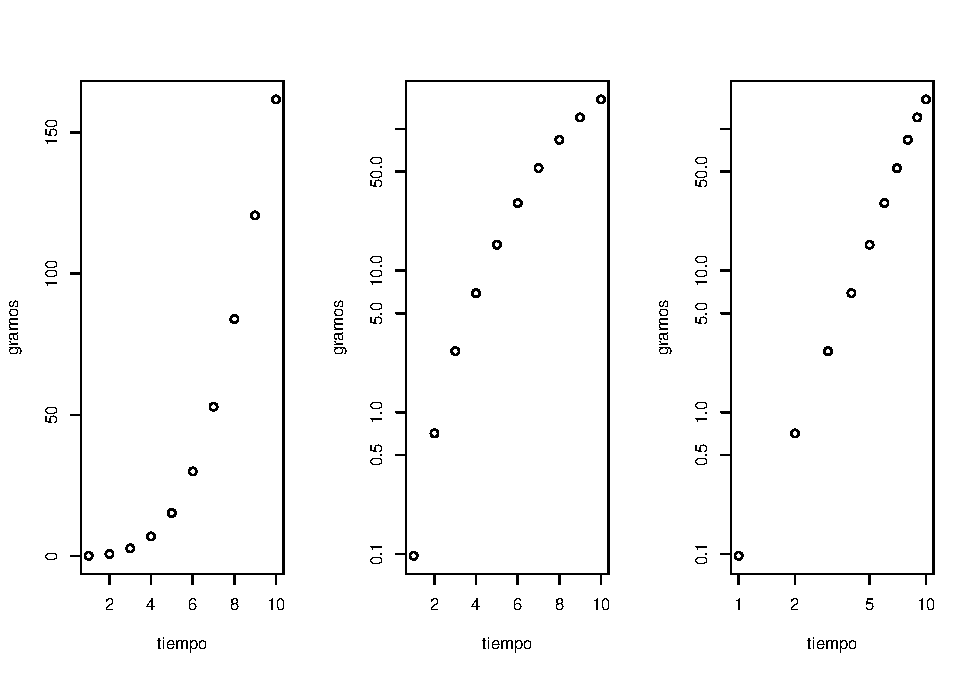
\includegraphics{Teoria4_files/figure-latex/unnamed-chunk-1-1.pdf}

\begin{Shaded}
\begin{Highlighting}[]
\FunctionTok{par}\NormalTok{(}\AttributeTok{mfrow=} \FunctionTok{c}\NormalTok{(}\DecValTok{1}\NormalTok{,}\DecValTok{1}\NormalTok{))}
\end{Highlighting}
\end{Shaded}

\hypertarget{las-distribuciones-de-probabilidad}{%
\section{Las distribuciones de
probabilidad}\label{las-distribuciones-de-probabilidad}}

\hypertarget{los-experimentos-aleatorios}{%
\subsection{Los experimentos
aleatorios}\label{los-experimentos-aleatorios}}

-Un experimento es un acto en el cual no conoces el resultado. -Un
suceso elemental son los posibles resultados. Cara o cruz. -El espacio
muestral es el conjunto de todos los sucesos elementales.

\hypertarget{variable-aleatoria}{%
\subsection{Variable Aleatoria}\label{variable-aleatoria}}

Es una variable que toma distintos valores. El dominio de la variable
aleatoria son todos los números que puede tomar.
\(p(X=a) = p(\{\omega\in\Omega \ |\  X(\omega) = a\})\)

Se lee: La probabilidad de que la variable aleatoria tome el valor a, es
la probabilidad de que el suceso (w) que pertenece al espacio muestral,
tal que X de w sea igual a a.

\begin{itemize}
\item
  \(p(a< X< b) = p(\{\omega\in\Omega \ |\  a< X(\omega) < b\})\)
\item
  \(p(X\in A) = p(\{\omega\in\Omega \ |\  X(\omega)\in A\})\)
\end{itemize}

\hypertarget{la-funciuxf3n-de-distribuciuxf3n}{%
\subsection{La función de
distribución}\label{la-funciuxf3n-de-distribuciuxf3n}}

Funcion de distribucion de la v.a. X. Es una funcion:
\[F:\mathbb{R}\longrightarrow [0,1]\]

dado por: \[F(x)=p(X\le x)\]

Que se lee como el valor acumulado \(F(x)\) es igual a la suma de todas
las probabilidades anteriores a x \(p(X\le x)\)

\hypertarget{ejemplo-tirar-un-dado-de-6-caras}{%
\subsubsection{Ejemplo tirar un dado de 6
caras}\label{ejemplo-tirar-un-dado-de-6-caras}}

Queremos saber la probabilidad de sacar 5. Es decir \(F(5)\) igual a la
probabilidad de que la v.a. tome el valor de 5, \(p(5\le x)\)

\hypertarget{variable-aleatoria-discreta}{%
\section{Variable Aleatoria
Discreta}\label{variable-aleatoria-discreta}}

-Una v.a es discreta cuando \(X:\Omega\longrightarrow\mathbb{R}\) y
\(D_x\) es finito, es decir el dominio de x es un subconjunto de los
naturales. La v.a. solo toma los valores de su dominio. Ejemplo las
caras de un dado, ya que este es un número finito.

-Funcion de densidad es la funcion \(f:\mathbb{R}\longrightarrow[0,1]\),
definido por \[f(x)=p(X=x)\]

Se concluye que \(f(x)=0\) si \(x\not\in D_x\). A lo cual llegamos que
la funcion de densidad es: \(f: D_x\longrightarrow[0,1]\)

\hypertarget{esperanza}{%
\subsubsection{Esperanza}\label{esperanza}}

Dado \(f: D_x\longrightarrow[0,1]\), entonces podemos decir que la
esperanza es la multiplicacion de cada elemento \(x\) dentro de \(D_x\)
por su probabilidad. \[E(X)=\sum_{x\in D_x}x \cdot f(x) \] Esta version
es muy parecida a la media vista como la sumatoria de la frecuencia
relativa por cada valor. Esto se vio en un documento pasado. Tambien se
ve como:

\[E(g(X))=\sum_{x\in D_x}g(x) \cdot f(x) \] Podemos calcular la
esperanza de \(x^2\) \[E(X^2)=\sum_{x\in D_x}x^2 \cdot f(x) \]

\hypertarget{varianza}{%
\subsubsection{Varianza}\label{varianza}}

Como vimos en capitulos pasados, la varianza es la diferencia de la
media de X al cuadrado menos el cuadrado de la media de x.En terminos se
esperanza es similar, se puede demostrar desde: \[Var(X)=E((X-E(X))^2)\]
Se entiende como la diferencia de X respecto a su valor esperado elevado
al cuadrado. Se resuelve como: \[=E(X^2-2XE(X)+E(X)^2)\]
\[=E(X^2)-E(2XE(X))+E(E(X)^2)\] El valor esperado en \(E(E(X)^2)\)
seguira siendo \(E(X)^2\) \[=E(X^2)-2E(X)E(X)+E(X)^2\]
\[=E(X^2)-2[E(X)]^2+E(X)^2\] \[Var(X)=E(X^2)-[E(X)]^2\] Tambien lo
podemos entender como: Si \(X\) es una v.a. discreta y
\(g:D_X\longrightarrow \mathbb{R}\) una función,
\[Var(g(X))=E((g(X)-E(g(X)))^2)=E(g(X)^2)-[E(g(X))]^2\] En este caso
\(g\) es una funcion cualquiera con un dominio de dicha variable
aleatoria discreta.

\hypertarget{desviacion-tipica}{%
\subsubsection{Desviacion tipica}\label{desviacion-tipica}}

Se entiende como: \[\sigma(X)=\sqrt{Var(X)}\] Tambien se puede entender
como: \[\sigma(g(X))=\sqrt{Var(g(X))}\]

\hypertarget{distribuciones-de-probabilidad-aplicadas}{%
\section{Distribuciones de probabilidad
aplicadas}\label{distribuciones-de-probabilidad-aplicadas}}

Cualquier variable aleatoria (va) se puede trabajar con las funciones
dva, pva, qva y rva.

-\textbf{dva} nos dara la función de densidad o probabilidad de la
variable. Su remplazo en python es pmf o pdf.

-\textbf{pva} nos dara la funcion de distribucion \(F(x)\) de la
variable aleatoria. Su remplazo en python es cdf.

-\textbf{qva} nos dara el cuartil de la variable. El valor minimo donde
\(F(x)\geq p\). Su remplazo en python es ppf.

-\textbf{rva} genera obserbacion con la distribucion de la variable
aleatoria. Su remplazo en python es rvs.

En R usamos Rlab y en python usamos scipy.stats

\hypertarget{distribucion-de-bernoulli}{%
\subsection{Distribucion de Bernoulli}\label{distribucion-de-bernoulli}}

Si X mide el numero de casos a favor o de exito, si se realiza un
experimento (1 en caso de exito y 0 en caso de fracaso). Si X sigue una
distribucion de Bernoulli con parametro p(probabilidad de exito)
utilizaremos: \[X\sim \text{Be}(p) \]

\hypertarget{elementos-importantes}{%
\subsubsection{Elementos importantes}\label{elementos-importantes}}

Donde la \textbf{probabilidad} de fracaso es \(q=1-p\).

El \textbf{dominio} de \(X\) es \(X(\Omega)=\{0,1\}\). Tambien se puede
entender como \(D_X = \{0,1\}\). Donde el dominio solo abarca 0 y 1,
entendido como fracaso y exito.

La \textbf{función de probabilidad} esta dada por:
\[f(k)=p^k(1-p)^{1-k}= \left\{
\begin{array}{rl}
     p & \text{si } k=1 
  \\ 1-p & \text{si } k=0
  \\ 0 & \text{en cualquier otro caso}
\end{array}
\right.\]

-Donde si \(k=1\) entonces
\(f(k)=p^1(1-p)^{1-1}=f(k)=p^1(1-p)^{0}\longrightarrow f(k)=p\)

-Donde si \(k=0\) entonces
\(f(k)=p^0(1-p)^{1-0}=f(k)=p^0(1-p)^{1}=1-p\longrightarrow f(k)=q\)

-Donde si toma otro valor sera cero, puesto que se trata de una
distribución discreta.

La \textbf{función de distribución acumulada} esta dada por:

\[F(k) = \left\{
\begin{array}{rl}
     0 & \text{si } k<0 
  \\ 1-p & \text{si } 0\le k<1
  \\ 1 & \text{si } k\ge 1
\end{array}
\right.\] Para los calculos de la media procedemos a remplazar \(k\) por
\(x\) La media de la distribucion de Bernoulli es:
\[E(X)=0*P(X=0)+1*P(X=1) \longrightarrow E(X)=P(X=1)=p\] La varianza de
la distribucion de Benoulli es: \[Var(X)=E(X^2)-E(X)^2\]
\[E(X^2)=\sum_{x=0}^1 x^2p^xq^{1-x}\]
\[E(X^2)=0^2p^0q^{1-0}+1^2p^1q^{1-1}\] \[E(X^2)=p^1q^{1-1}=p\]

Por lo tanto podemos retomar: \[Var(X)=p-p^2=p(1-p)\]

\hypertarget{corriendo-la-distribucion-de-bernoulli}{%
\subsubsection{Corriendo la distribucion de
Bernoulli}\label{corriendo-la-distribucion-de-bernoulli}}

\textbf{Funcion de densidad o de probabilidad}
\[f(x)=p^x(1-p)^{1-x}, k={0,1}\] Suponiendo que tenemos una moneda
trucada con probabilidad de exito de 0.7. Es decir
\(X\sim \text{Be}\ (p=0.7)\)

\begin{Shaded}
\begin{Highlighting}[]
\FunctionTok{library}\NormalTok{(Rlab)}
\end{Highlighting}
\end{Shaded}

\begin{verbatim}
## Rlab 4.0 attached.
\end{verbatim}

\begin{verbatim}
## 
## Attaching package: 'Rlab'
\end{verbatim}

\begin{verbatim}
## The following objects are masked from 'package:stats':
## 
##     dexp, dgamma, dweibull, pexp, pgamma, pweibull, qexp, qgamma,
##     qweibull, rexp, rgamma, rweibull
\end{verbatim}

\begin{verbatim}
## The following object is masked from 'package:datasets':
## 
##     precip
\end{verbatim}

\begin{Shaded}
\begin{Highlighting}[]
\FunctionTok{dbern}\NormalTok{(}\DecValTok{0}\NormalTok{,}\FloatTok{0.7}\NormalTok{) }\CommentTok{\#dbern trabaja la distribucion de Bernoulli}
\end{Highlighting}
\end{Shaded}

\begin{verbatim}
## [1] 0.3
\end{verbatim}

\begin{Shaded}
\begin{Highlighting}[]
\FunctionTok{dbern}\NormalTok{(}\DecValTok{1}\NormalTok{,}\FloatTok{0.7}\NormalTok{)}
\end{Highlighting}
\end{Shaded}

\begin{verbatim}
## [1] 0.7
\end{verbatim}

\begin{Shaded}
\begin{Highlighting}[]
\FunctionTok{pbern}\NormalTok{(}\DecValTok{0}\NormalTok{,}\FloatTok{0.7}\NormalTok{)}
\end{Highlighting}
\end{Shaded}

\begin{verbatim}
## [1] 0.3
\end{verbatim}

\begin{Shaded}
\begin{Highlighting}[]
\FunctionTok{pbern}\NormalTok{(}\DecValTok{1}\NormalTok{,}\FloatTok{0.7}\NormalTok{)}
\end{Highlighting}
\end{Shaded}

\begin{verbatim}
## [1] 1
\end{verbatim}

\begin{Shaded}
\begin{Highlighting}[]
\FunctionTok{qbern}\NormalTok{(}\FloatTok{0.5}\NormalTok{,}\FloatTok{0.7}\NormalTok{)}
\end{Highlighting}
\end{Shaded}

\begin{verbatim}
## [1] 1
\end{verbatim}

\begin{Shaded}
\begin{Highlighting}[]
\FunctionTok{qbern}\NormalTok{(}\FloatTok{0.25}\NormalTok{,}\FloatTok{0.7}\NormalTok{)}
\end{Highlighting}
\end{Shaded}

\begin{verbatim}
## [1] 0
\end{verbatim}

\begin{Shaded}
\begin{Highlighting}[]
\FunctionTok{rbern}\NormalTok{(}\DecValTok{100}\NormalTok{,}\FloatTok{0.7}\NormalTok{)}\OtherTok{{-}\textgreater{}}\NormalTok{data}
\FunctionTok{hist}\NormalTok{(data)}
\end{Highlighting}
\end{Shaded}

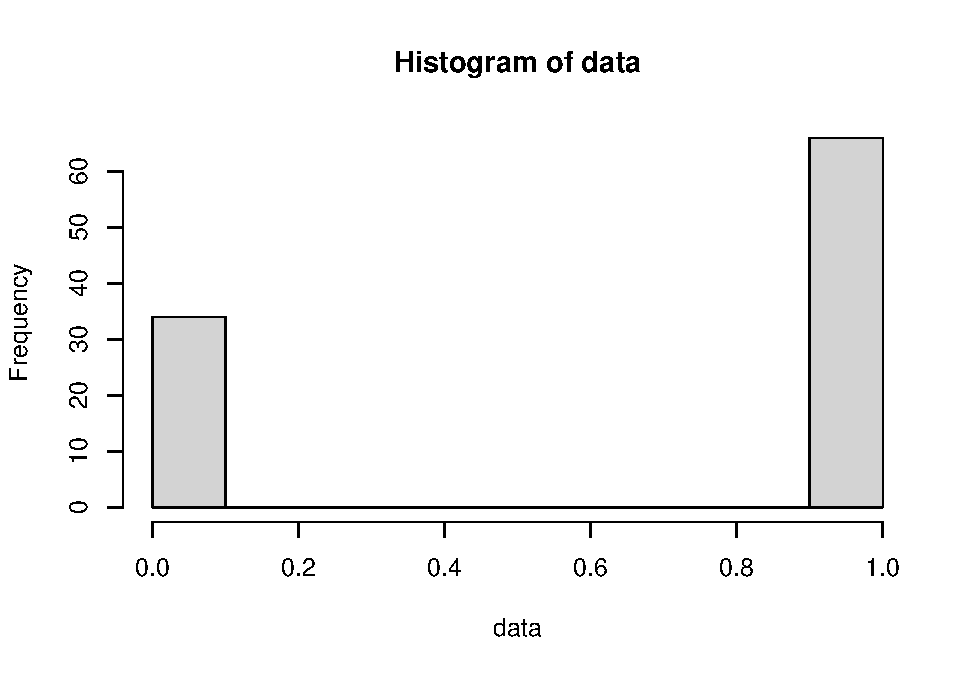
\includegraphics{Teoria4_files/figure-latex/Primeros experimentos-1.pdf}
Nos arroja que la probabilidad de sacar 0 es de 0.3 y la de sacar 1 es
de 0.7

\hypertarget{distribucion-binomial}{%
\subsection{Distribucion Binomial}\label{distribucion-binomial}}

Si \(X\) es una V.A. la cual mide el numero de exitos donde se realizan
\(n\) ensayos de Bernoulli independientes entre si, entonces \(X\) se
distribuye de la siguiente forma. \[X\sim \text{B}(n,p)\]

El dominio sera \(D_X = \{0,1,2,\dots,n\}\) La funcion de densidad
estara dada por: \[f(k) = {n\choose k}p^k(1-p)^{n-k} \] - La
\textbf{función de distribución} (probabilidad acumulada) vendrá dada
por \[F(x) = \left\{
\begin{array}{cl}
     0 & \text{si } x<0 
  \\ \sum_{k=0}^xf(k) & \text{si } 0\le x<n
  \\ 1 & \text{si } x\ge n
\end{array}
\right.\]

\begin{itemize}
\tightlist
\item
  \textbf{Esperanza} \(E(X) = np\)
\item
  \textbf{Varianza} \(Var(X) = npq\)
\end{itemize}

\begin{Shaded}
\begin{Highlighting}[]
\FunctionTok{plot}\NormalTok{(}\DecValTok{0}\SpecialCharTok{:}\DecValTok{50}\NormalTok{,}\FunctionTok{dbinom}\NormalTok{(}\DecValTok{0}\SpecialCharTok{:}\DecValTok{50}\NormalTok{,}\DecValTok{50}\NormalTok{,}\FloatTok{0.5}\NormalTok{),}\AttributeTok{col =} \StringTok{"purple"}\NormalTok{, }\AttributeTok{xlab =} \StringTok{""}\NormalTok{, }\AttributeTok{ylab =} \StringTok{""}\NormalTok{, }\AttributeTok{main =} \StringTok{"Función de probabilidad de una B(50,0.5)"}\NormalTok{)}
\end{Highlighting}
\end{Shaded}

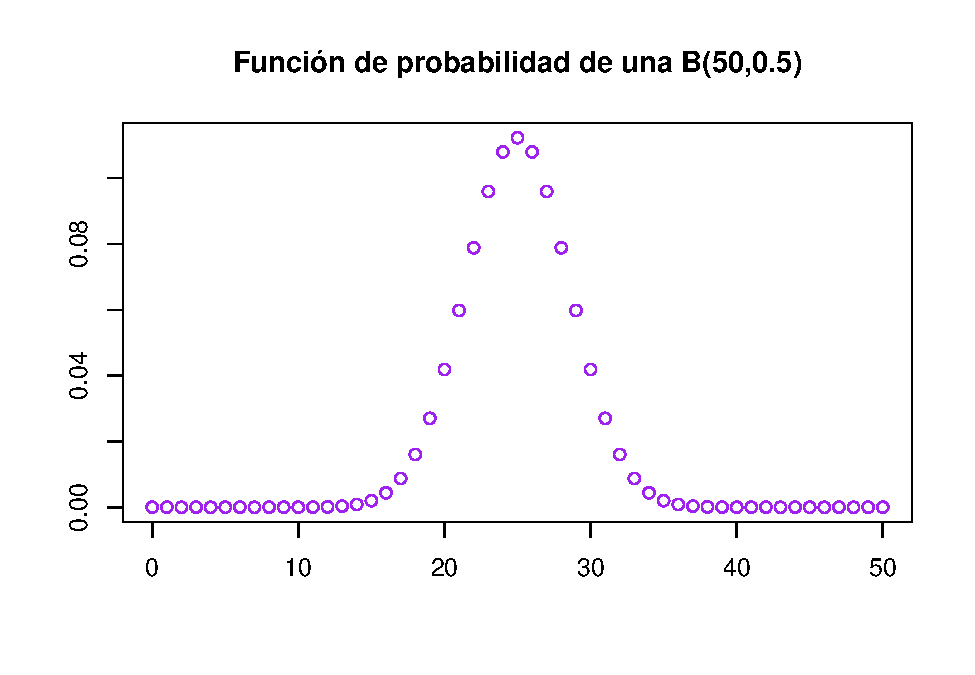
\includegraphics{Teoria4_files/figure-latex/Ejemplos de distribucion binomial-1.pdf}

\begin{Shaded}
\begin{Highlighting}[]
\FunctionTok{plot}\NormalTok{(}\DecValTok{0}\SpecialCharTok{:}\DecValTok{50}\NormalTok{, }\FunctionTok{pbinom}\NormalTok{(}\DecValTok{0}\SpecialCharTok{:}\DecValTok{50}\NormalTok{,}\DecValTok{50}\NormalTok{,}\FloatTok{0.5}\NormalTok{),}\AttributeTok{col =} \StringTok{"purple"}\NormalTok{, }\AttributeTok{xlab =} \StringTok{""}\NormalTok{, }\AttributeTok{ylab =} \StringTok{""}\NormalTok{, }\AttributeTok{main =} \StringTok{"Función de distribución de una B(50,0.5)"}\NormalTok{, }\AttributeTok{ylim =} \FunctionTok{c}\NormalTok{(}\DecValTok{0}\NormalTok{,}\DecValTok{1}\NormalTok{))}
\end{Highlighting}
\end{Shaded}

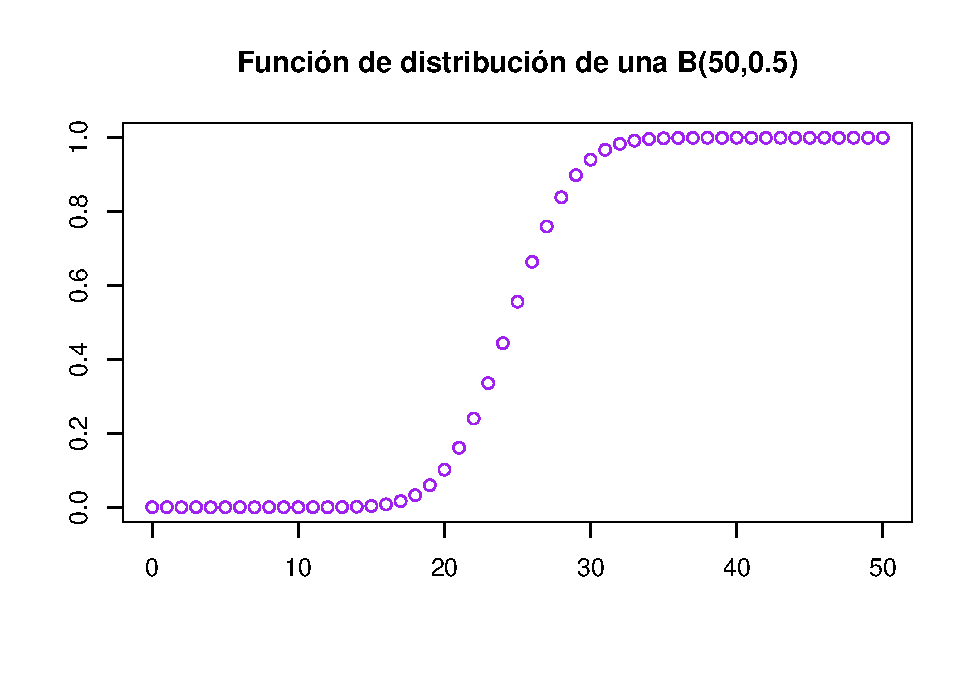
\includegraphics{Teoria4_files/figure-latex/Ejemplos de distribucion binomial-2.pdf}

\hypertarget{ejemplo}{%
\subsubsection{Ejemplo}\label{ejemplo}}

Sea \(X = B(30, 0.6)\)

\begin{Shaded}
\begin{Highlighting}[]
\NormalTok{n}\OtherTok{\textless{}{-}}\DecValTok{30}
\NormalTok{p}\OtherTok{\textless{}{-}}\FloatTok{0.6}
\NormalTok{x}\OtherTok{\textless{}{-}}\DecValTok{0}\SpecialCharTok{:}\DecValTok{30}
\CommentTok{\#FUncion de densidad}
\NormalTok{ejemplobinomial}\OtherTok{\textless{}{-}}\FunctionTok{dbinom}\NormalTok{(x, n, p)}
\FunctionTok{plot}\NormalTok{(ejemplobinomial)}
\end{Highlighting}
\end{Shaded}

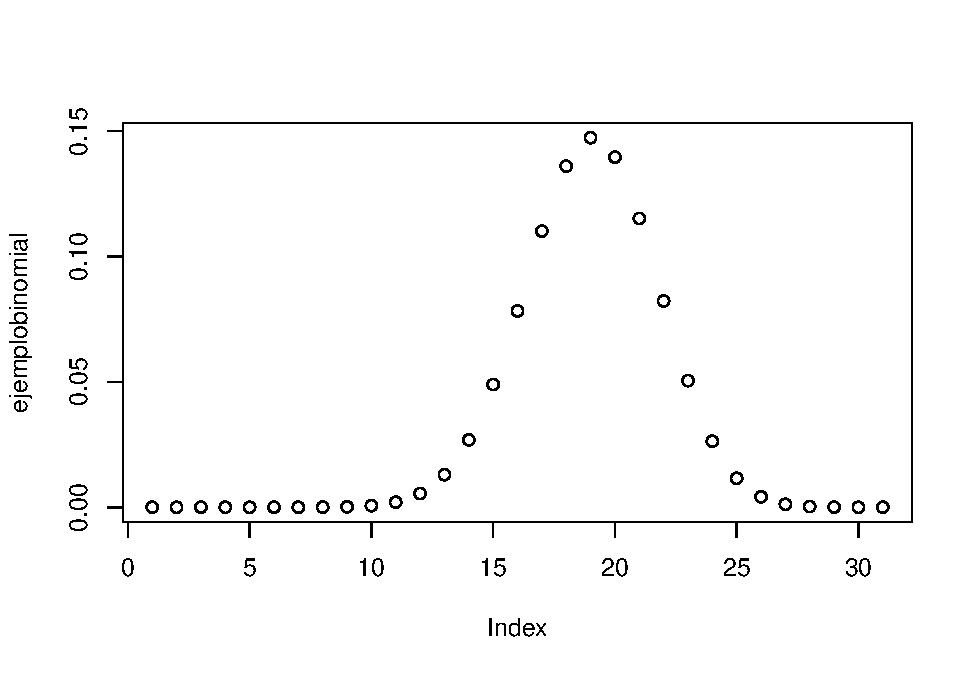
\includegraphics{Teoria4_files/figure-latex/unnamed-chunk-2-1.pdf}

\begin{Shaded}
\begin{Highlighting}[]
\NormalTok{media\_ejemplobinomial}\OtherTok{\textless{}{-}}\NormalTok{n}\SpecialCharTok{*}\NormalTok{p}
\NormalTok{var\_ejemplobinomial}\OtherTok{\textless{}{-}}\NormalTok{n}\SpecialCharTok{*}\NormalTok{p}\SpecialCharTok{*}\NormalTok{(}\DecValTok{1}\SpecialCharTok{{-}}\NormalTok{p)}
\NormalTok{media\_ejemplobinomial}
\end{Highlighting}
\end{Shaded}

\begin{verbatim}
## [1] 18
\end{verbatim}

\begin{Shaded}
\begin{Highlighting}[]
\NormalTok{var\_ejemplobinomial}
\end{Highlighting}
\end{Shaded}

\begin{verbatim}
## [1] 7.2
\end{verbatim}

\begin{Shaded}
\begin{Highlighting}[]
\CommentTok{\#Funcion de distribucion}
\NormalTok{ejemplobinomial\_acu}\OtherTok{\textless{}{-}}\FunctionTok{pbinom}\NormalTok{(x, n, p)}
\FunctionTok{plot}\NormalTok{(ejemplobinomial\_acu)}
\end{Highlighting}
\end{Shaded}

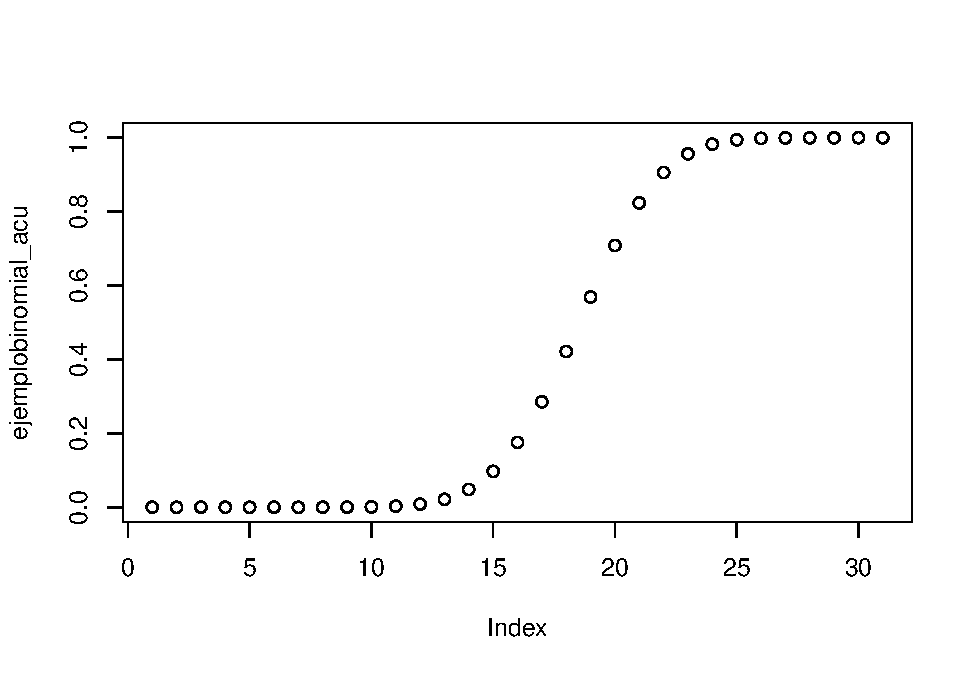
\includegraphics{Teoria4_files/figure-latex/unnamed-chunk-2-2.pdf}

\begin{Shaded}
\begin{Highlighting}[]
\FunctionTok{qbinom}\NormalTok{(}\FloatTok{0.5}\NormalTok{,n,p)}
\end{Highlighting}
\end{Shaded}

\begin{verbatim}
## [1] 18
\end{verbatim}

\begin{Shaded}
\begin{Highlighting}[]
\FunctionTok{hist}\NormalTok{(}\FunctionTok{rbinom}\NormalTok{(}\DecValTok{100}\NormalTok{,n,p)) }\CommentTok{\#Parece tener sesgo cuando hacemos 100 repeticiones}
\end{Highlighting}
\end{Shaded}

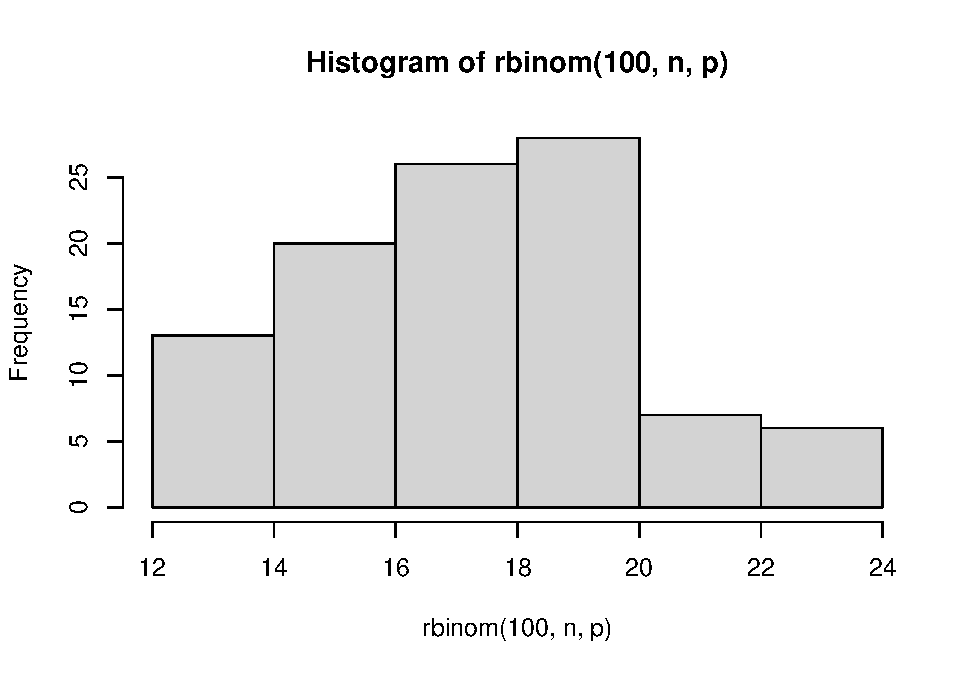
\includegraphics{Teoria4_files/figure-latex/unnamed-chunk-2-3.pdf} El
50\% esta debajo de 18.

\hypertarget{distribucion-geometrica}{%
\subsection{Distribucion Geometrica}\label{distribucion-geometrica}}

Si X es una variable que se encarga de medir el ``numero de repeticiones
independientes del experimento hasta conseguir exito'' se distribuira de
la siguiente forma. \[X\sim \text{Ge}(p)\] - El \textbf{dominio} de
\(X\) será \(D_X= \{0,1,2,\dots\}\) o bien \(D_X = \{1,2,\dots\}\) en
función de si empieza en 0 o en 1, respectivamente

\begin{itemize}
\tightlist
\item
  La \textbf{función de probabilidad o densidad} vendrá dada por
  \[f(k) = (1-p)^{k}p \qquad\text{ si empieza en 0}\]
\end{itemize}

\[f(k) = (1-p)^{k-1}p \qquad\text{ si empieza en 1}\] - La
\textbf{función de distribución} vendrá dada por \[F(x) = \left\{
\begin{array}{cl}
     0 & \text{si } x<0 
  \\ 1-(1-p)^{k+1} & \text{si } k\le x<k+1,\ k\in\mathbb{N}
\end{array}
\right.\]

\begin{itemize}
\tightlist
\item
  \textbf{Esperanza} \(E(X) = \frac{1-p}{p}\) si empieza en 0 y
  E\((X) = \frac{1}{p}\) si empieza en 1
\item
  \textbf{Varianza} \(Var(X) = \frac{1-p}{p^2}\)
\item
  Propiedad de la falta de memoria. Si \(X\) es una v.a.
  \(\text{Ge}(p)\), entonces,
  \[p\{X\ge m+n:\ X\ge n\} = p\{X\ge m\}\ \forall m,n=0,1,\dots\]
\end{itemize}

\begin{Shaded}
\begin{Highlighting}[]
\FunctionTok{par}\NormalTok{(}\AttributeTok{mfrow =} \FunctionTok{c}\NormalTok{(}\DecValTok{1}\NormalTok{,}\DecValTok{2}\NormalTok{))}
\FunctionTok{plot}\NormalTok{(}\DecValTok{0}\SpecialCharTok{:}\DecValTok{20}\NormalTok{, }\FunctionTok{dgeom}\NormalTok{(}\DecValTok{0}\SpecialCharTok{:}\DecValTok{20}\NormalTok{,}\FloatTok{0.5}\NormalTok{),}\AttributeTok{col =} \StringTok{"purple"}\NormalTok{, }\AttributeTok{xlab =} \StringTok{""}\NormalTok{, }\AttributeTok{ylab =} \StringTok{""}\NormalTok{, }\AttributeTok{main =} \StringTok{"Función de probabilidad de una Ge(0.5)"}\NormalTok{)}
\FunctionTok{plot}\NormalTok{(}\DecValTok{0}\SpecialCharTok{:}\DecValTok{20}\NormalTok{, }\FunctionTok{pgeom}\NormalTok{(}\DecValTok{0}\SpecialCharTok{:}\DecValTok{20}\NormalTok{,}\FloatTok{0.5}\NormalTok{),}\AttributeTok{col =} \StringTok{"purple"}\NormalTok{, }\AttributeTok{xlab =} \StringTok{""}\NormalTok{, }\AttributeTok{ylab =} \StringTok{""}\NormalTok{, }\AttributeTok{main =} \StringTok{"Función de distribución de una Ge(0.5)"}\NormalTok{, }\AttributeTok{ylim =} \FunctionTok{c}\NormalTok{(}\DecValTok{0}\NormalTok{,}\DecValTok{1}\NormalTok{))}
\end{Highlighting}
\end{Shaded}

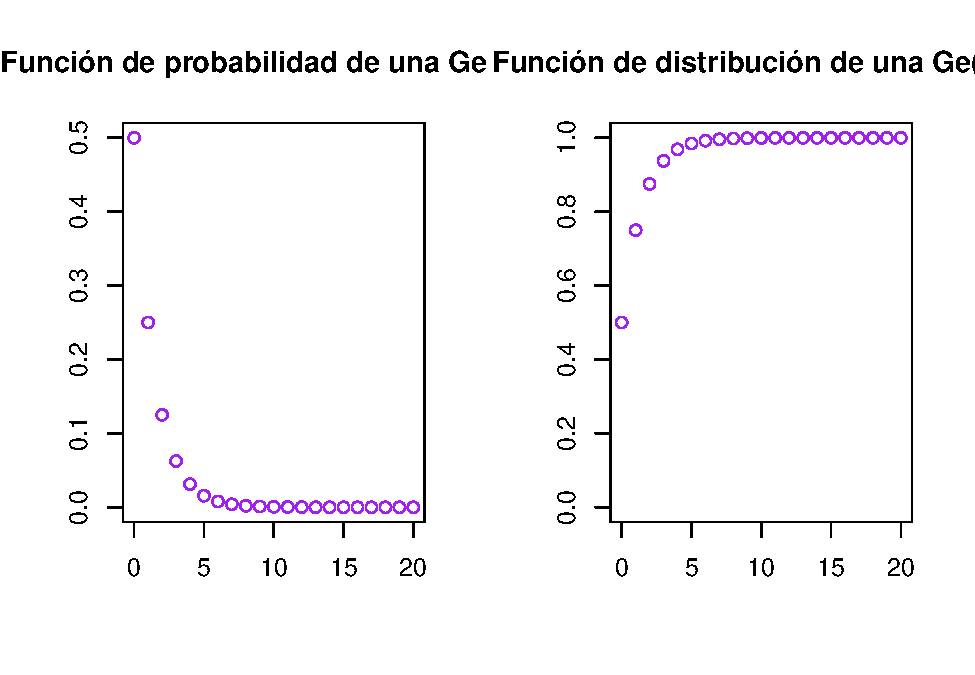
\includegraphics{Teoria4_files/figure-latex/Distribucion Geometrica-1.pdf}

\begin{Shaded}
\begin{Highlighting}[]
\FunctionTok{par}\NormalTok{(}\AttributeTok{mfrow=} \FunctionTok{c}\NormalTok{(}\DecValTok{1}\NormalTok{,}\DecValTok{1}\NormalTok{))}
\end{Highlighting}
\end{Shaded}

completar

\hypertarget{distribucion-de-poisson}{%
\subsection{Distribucion de Poisson}\label{distribucion-de-poisson}}

La V.A. \(X\) se encarga de medir el numero de eventos en determinado
tiempo y sigue la distribucion: \[X\sim \text{Po}(\lambda)\] Donde
\(\lambda\) es el numero de veces que ocurre el evento en el momento
especificado. - El \textbf{dominio} de \(X\) será
\(D_X = \{0,1,2,\dots\}\)

\begin{itemize}
\item
  La \textbf{función de probabilidad} vendrá dada por
  \[f(k) = \frac{e^{-\lambda}\lambda^k}{k!}\]
\item
  La \textbf{función de distribución} vendrá dada por \[F(x) = \left\{
  \begin{array}{cl}
     0 & \text{si } x<0 
  \\ \sum_{k=0}^xf(k) & \text{si } 0\le x<n
  \\ 1 & \text{si } x\ge n
  \end{array}
  \right.\]
\item
  \textbf{Esperanza} \(E(X) = \lambda\)
\item
  \textbf{Varianza} \(Var(X) = \lambda\)
\end{itemize}

\begin{Shaded}
\begin{Highlighting}[]
\FunctionTok{plot}\NormalTok{(}\DecValTok{0}\SpecialCharTok{:}\DecValTok{20}\NormalTok{, }\FunctionTok{dpois}\NormalTok{(}\DecValTok{0}\SpecialCharTok{:}\DecValTok{20}\NormalTok{,}\DecValTok{2}\NormalTok{),}\AttributeTok{col =} \StringTok{"purple"}\NormalTok{, }\AttributeTok{xlab =} \StringTok{""}\NormalTok{, }\AttributeTok{ylab =} \StringTok{""}\NormalTok{, }\AttributeTok{main =} \StringTok{"Función de probabilidad de una Po(2)"}\NormalTok{)}
\end{Highlighting}
\end{Shaded}

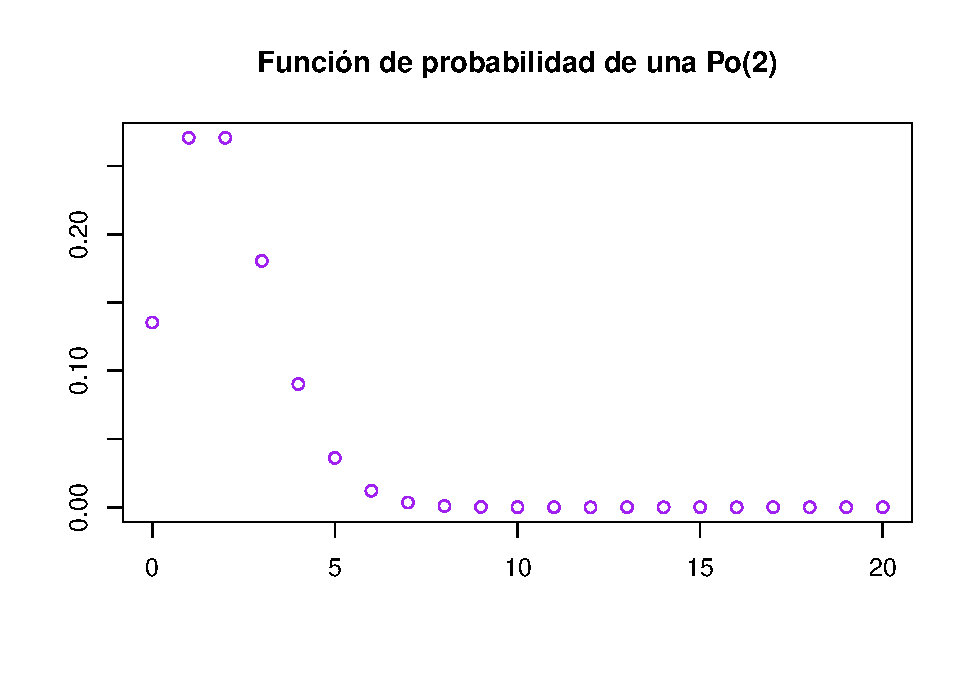
\includegraphics{Teoria4_files/figure-latex/Distribucion de Poisson-1.pdf}

\begin{Shaded}
\begin{Highlighting}[]
\FunctionTok{plot}\NormalTok{(}\DecValTok{0}\SpecialCharTok{:}\DecValTok{20}\NormalTok{, }\FunctionTok{ppois}\NormalTok{(}\DecValTok{0}\SpecialCharTok{:}\DecValTok{20}\NormalTok{,}\DecValTok{2}\NormalTok{),}\AttributeTok{col =} \StringTok{"purple"}\NormalTok{, }\AttributeTok{xlab =} \StringTok{""}\NormalTok{, }\AttributeTok{ylab =} \StringTok{""}\NormalTok{, }\AttributeTok{main =} \StringTok{"Función de distribución de una Po(2)"}\NormalTok{, }\AttributeTok{ylim =} \FunctionTok{c}\NormalTok{(}\DecValTok{0}\NormalTok{,}\DecValTok{1}\NormalTok{))}
\end{Highlighting}
\end{Shaded}

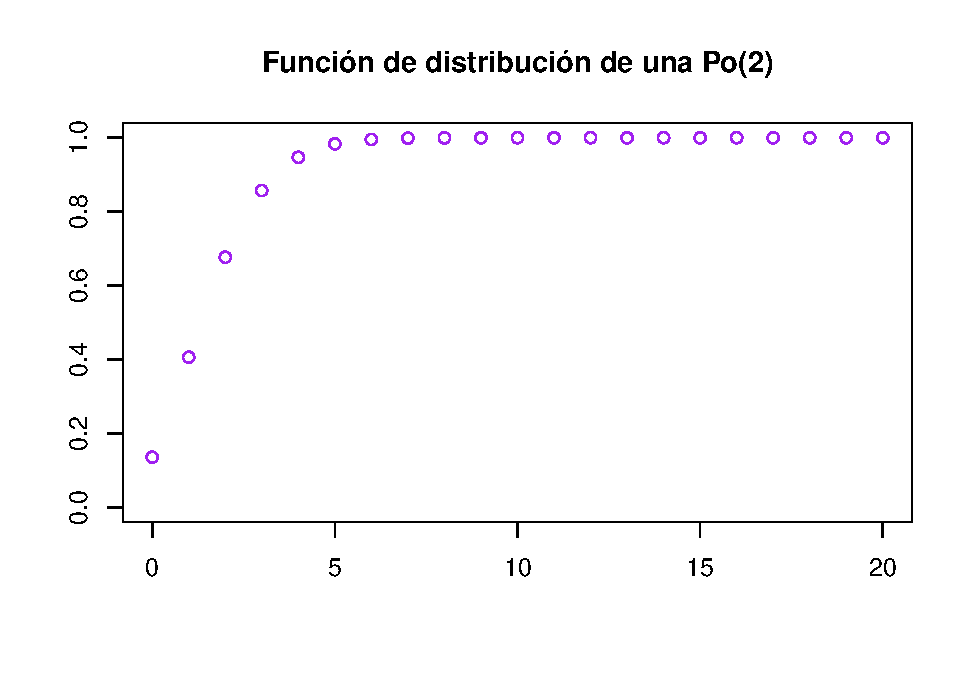
\includegraphics{Teoria4_files/figure-latex/Distribucion de Poisson-2.pdf}
Ejemplo de \(\lambda=5\)

\begin{Shaded}
\begin{Highlighting}[]
\NormalTok{l}\OtherTok{=}\DecValTok{5}
\NormalTok{x}\OtherTok{\textless{}{-}}\DecValTok{0}\SpecialCharTok{:}\DecValTok{30}
\NormalTok{distr\_poisson }\OtherTok{\textless{}{-}} \FunctionTok{dpois}\NormalTok{(x,l)}
\NormalTok{distr\_poisson}
\end{Highlighting}
\end{Shaded}

\begin{verbatim}
##  [1] 6.737947e-03 3.368973e-02 8.422434e-02 1.403739e-01 1.754674e-01
##  [6] 1.754674e-01 1.462228e-01 1.044449e-01 6.527804e-02 3.626558e-02
## [11] 1.813279e-02 8.242177e-03 3.434240e-03 1.320862e-03 4.717363e-04
## [16] 1.572454e-04 4.913920e-05 1.445271e-05 4.014640e-06 1.056484e-06
## [21] 2.641211e-07 6.288597e-08 1.429227e-08 3.107014e-09 6.472947e-10
## [26] 1.294589e-10 2.489595e-11 4.610361e-12 8.232787e-13 1.419446e-13
## [31] 2.365743e-14
\end{verbatim}

\begin{Shaded}
\begin{Highlighting}[]
\FunctionTok{plot}\NormalTok{(distr\_poisson)}
\end{Highlighting}
\end{Shaded}

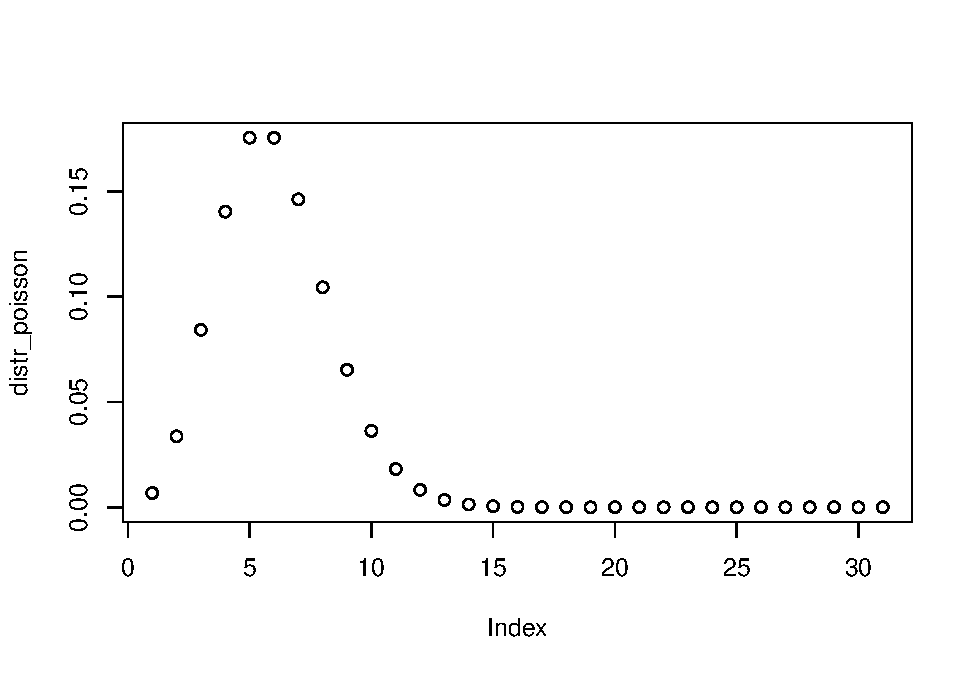
\includegraphics{Teoria4_files/figure-latex/Ejemplo de Poisson-1.pdf}

\begin{Shaded}
\begin{Highlighting}[]
\FunctionTok{hist}\NormalTok{(distr\_poisson)}
\end{Highlighting}
\end{Shaded}

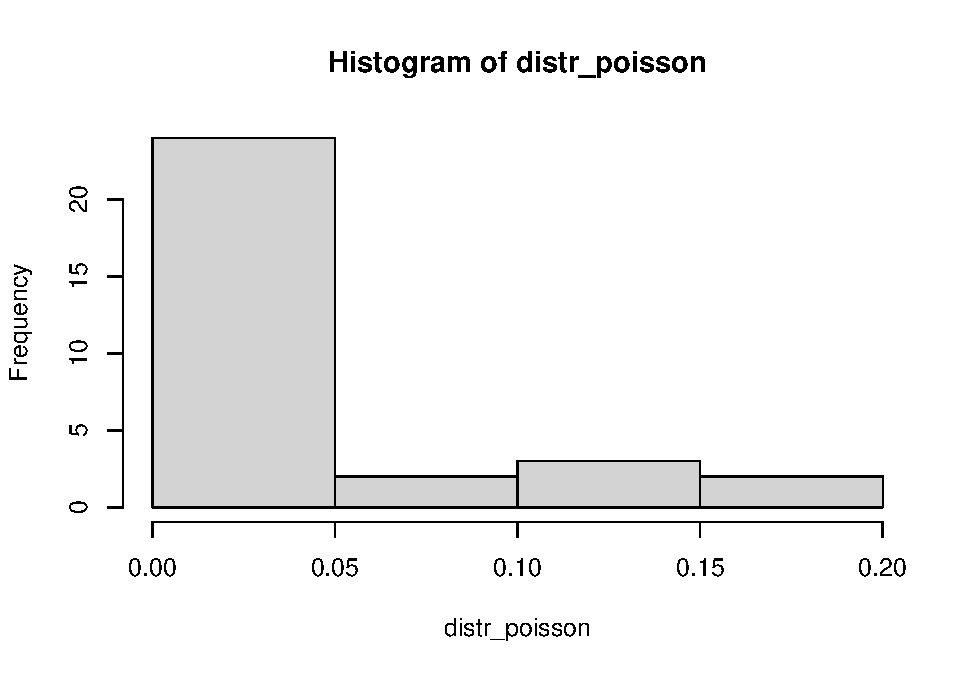
\includegraphics{Teoria4_files/figure-latex/Ejemplo de Poisson-2.pdf}

\hypertarget{variable-aleatoria-continua}{%
\section{Variable Aleatoria
Continua}\label{variable-aleatoria-continua}}

Una V.A. es continua cuando hay numeros continuos en \([0,1]\)

\textbf{Función de densidad}

Función de densidad. Función \(f:\mathbb{R}\longrightarrow\mathbb{R}\)
que satisface

\begin{itemize}
\tightlist
\item
  \(f(x)\ge 0\ \forall x\in\mathbb{R}\)
\item
  \(\int_{-\infty}^{+\infty}f(t)dt=1\)
\end{itemize}

Una función de densidad puede tener puntos de discontinuidad. Mientras
el area bajo la curva sea de 1 estaremos hablando de una funcion de
densidad.

\hypertarget{esperanza-1}{%
\subsection{Esperanza}\label{esperanza-1}}

Esperanza de una v.a. continua. Sea \(X\) v.a. continua con densidad
\(f_X\). La esperanza de \(X\) es
\[E(X)=\int_{-\infty}^{+\infty}x\cdot f_X(x)dx\]

Si el dominio \(D_X\) de \(X\) es un intervalo de extremos \(a<b\),
entonces \[E(X)=\int_a^b x\cdot f_X(x)dx\]

\hypertarget{esperanza-2}{%
\subsection{Esperanza}\label{esperanza-2}}

Sea \(g:D_X\longrightarrow \mathbb{R}\) una función continua. Entonces,

\[E(g(X)) = \int_{-\infty}^{+\infty}g(x)\cdot f_X(x)dx\] Si el dominio
\(D_X\) de \(X\) es un intervalo de extremos \(a<b\), entonces
\[E(g(X))=\int_a^b g(x)\cdot f_X(x)dx\]

\hypertarget{varianza-1}{%
\subsection{Varianza}\label{varianza-1}}

Varianza de una v.a. continua. Como en el caso discreto,
\[Var(X)=E((X-E(X))^2)\]

y se puede demostrar que

\[Var(X)=E(X^2)-(E(X))^2\]

\hypertarget{distribuciones-continuas}{%
\subsection{Distribuciones continuas}\label{distribuciones-continuas}}

\begin{Shaded}
\begin{Highlighting}[]
\CommentTok{\#[Uniforme](https://es.wikipedia.org/wiki/Distribución\_uniforme\_continua)}
\CommentTok{\#[Exponencial](https://es.wikipedia.org/wiki/Distribución\_exponencial)}
\CommentTok{\#[Normal](https://es.wikipedia.org/wiki/Distribución\_normal)}
\CommentTok{\#[Khi cuadrado](https://es.wikipedia.org/wiki/Distribución\_χ²)}
\CommentTok{\#[t de Student](https://es.wikipedia.org/wiki/Distribución\_t\_de\_Student)}
\CommentTok{\#[F de Fisher](https://es.wikipedia.org/wiki/Distribución\_F)}
\end{Highlighting}
\end{Shaded}

\hypertarget{distribuciuxf3n-uniforme}{%
\subsection{Distribución Uniforme}\label{distribuciuxf3n-uniforme}}

Una V.A. continua es uniforme cuando tiene una distribucion sobre el
intervalo real \([a,b]\) si \(a<b\), entonces sigue
\(X\sim\text{U}(a,b)\) \[f_X(x)=\left\{
\begin{array}{rl}
     \frac{1}{b-a} & \text{si } a\le x\le b
  \\ 0 & \text{en cualquier otro caso}
\end{array}
\right.\] Vemos que la probabilidad de estar en el intervalo es
constante. - El \textbf{dominio} de \(X\) será \(D_X = [a,b]\)

\begin{itemize}
\item
  La \textbf{función de distribución} vendrá dada por \[F_X(x)=\left\{
  \begin{array}{rl}
    0 & \text{si } x<a
  \\ \frac{x-a}{b-a} & \text{si } a\le x< b
  \\ 1 & \text{si } x\ge b
  \end{array}
  \right.\]
\item
  \textbf{Esperanza} \(E(X) = \frac{a+b}{2}\)
\item
  \textbf{Varianza} \(Var(X) = \frac{(b-a)^2}{12}\)
\end{itemize}

\begin{Shaded}
\begin{Highlighting}[]
\FunctionTok{plot}\NormalTok{(}\FunctionTok{c}\NormalTok{(}\DecValTok{0}\NormalTok{,}\DecValTok{1}\NormalTok{,}\DecValTok{1}\SpecialCharTok{:}\DecValTok{4}\NormalTok{,}\DecValTok{4}\NormalTok{,}\DecValTok{5}\NormalTok{), }\FunctionTok{c}\NormalTok{(}\DecValTok{0}\NormalTok{,}\DecValTok{0}\NormalTok{,}\FunctionTok{dunif}\NormalTok{(}\DecValTok{1}\SpecialCharTok{:}\DecValTok{4}\NormalTok{,}\AttributeTok{min =} \DecValTok{1}\NormalTok{, }\AttributeTok{max =} \DecValTok{4}\NormalTok{),}\DecValTok{0}\NormalTok{,}\DecValTok{0}\NormalTok{),}\AttributeTok{col =} \StringTok{"purple"}\NormalTok{, }\AttributeTok{xlab =} \StringTok{""}\NormalTok{, }\AttributeTok{ylab =} \StringTok{""}\NormalTok{, }\AttributeTok{main =} \StringTok{"Función de densidad de una U(1,4)"}\NormalTok{, }\AttributeTok{type =} \StringTok{"o"}\NormalTok{, }\AttributeTok{ylim =} \FunctionTok{c}\NormalTok{(}\DecValTok{0}\NormalTok{,}\DecValTok{1}\NormalTok{))}
\end{Highlighting}
\end{Shaded}

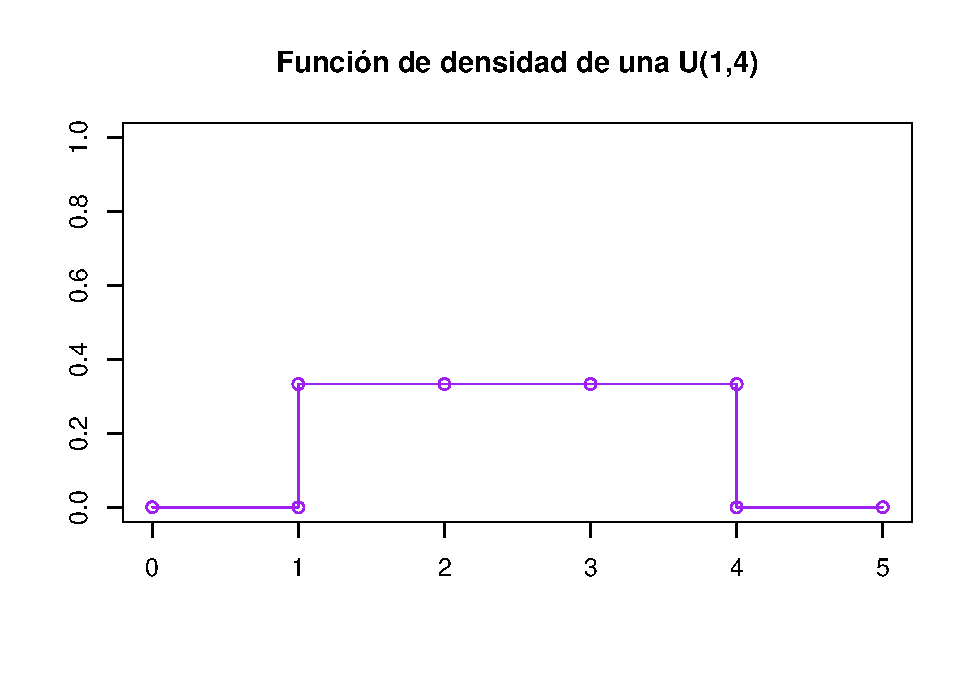
\includegraphics{Teoria4_files/figure-latex/Distribucion uniforme-1.pdf}

\begin{Shaded}
\begin{Highlighting}[]
\FunctionTok{plot}\NormalTok{(}\DecValTok{0}\SpecialCharTok{:}\DecValTok{5}\NormalTok{, }\FunctionTok{punif}\NormalTok{(}\DecValTok{0}\SpecialCharTok{:}\DecValTok{5}\NormalTok{,}\AttributeTok{min =} \DecValTok{1}\NormalTok{, }\AttributeTok{max =} \DecValTok{4}\NormalTok{),}\AttributeTok{col =} \StringTok{"purple"}\NormalTok{, }\AttributeTok{xlab =} \StringTok{""}\NormalTok{, }\AttributeTok{ylab =} \StringTok{""}\NormalTok{, }\AttributeTok{main =} \StringTok{"Función de distribución de una U(1,4)"}\NormalTok{, }\AttributeTok{type =} \StringTok{"o"}\NormalTok{)}
\end{Highlighting}
\end{Shaded}

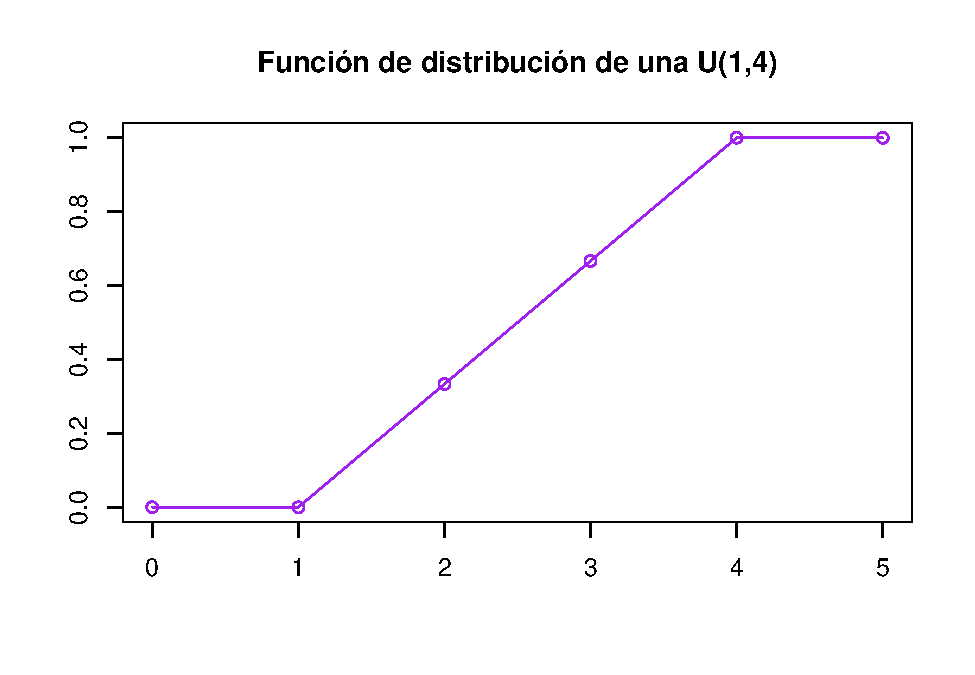
\includegraphics{Teoria4_files/figure-latex/Distribucion uniforme-2.pdf}

Supongamos el clasico caso, \(X\sim U(0,1)\), podemos modelar:

\begin{Shaded}
\begin{Highlighting}[]
\NormalTok{a}\OtherTok{=}\DecValTok{0}
\NormalTok{b}\OtherTok{=}\DecValTok{1}
\NormalTok{q}\OtherTok{=}\FloatTok{0.5}
\NormalTok{x}\OtherTok{\textless{}{-}}\FunctionTok{seq}\NormalTok{(}\SpecialCharTok{{-}}\FloatTok{0.1}\NormalTok{,}\FloatTok{1.1}\NormalTok{,}\FloatTok{0.1}\NormalTok{)}

\NormalTok{dens\_uni}\OtherTok{\textless{}{-}}\FunctionTok{dunif}\NormalTok{(x,a,b)}
\NormalTok{distr\_uni}\OtherTok{\textless{}{-}}\FunctionTok{punif}\NormalTok{(x,a,b)}
\FunctionTok{plot}\NormalTok{(dens\_uni)}
\end{Highlighting}
\end{Shaded}

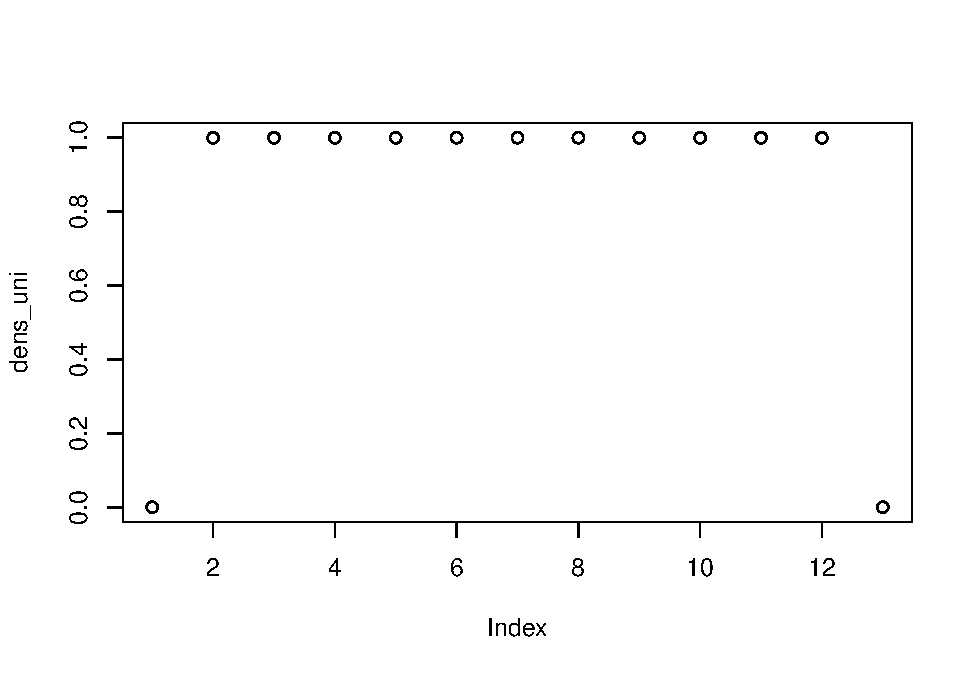
\includegraphics{Teoria4_files/figure-latex/Ejemplo distribucion uniforme-1.pdf}

\begin{Shaded}
\begin{Highlighting}[]
\FunctionTok{plot}\NormalTok{(distr\_uni)}
\end{Highlighting}
\end{Shaded}

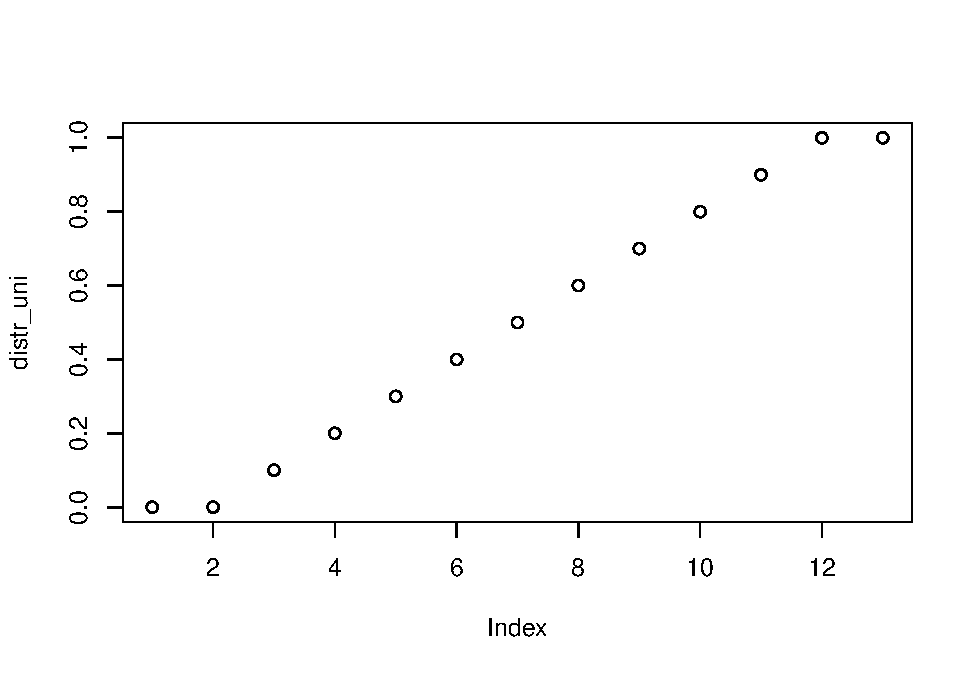
\includegraphics{Teoria4_files/figure-latex/Ejemplo distribucion uniforme-2.pdf}

\begin{Shaded}
\begin{Highlighting}[]
\FunctionTok{runif}\NormalTok{(}\DecValTok{1000}\NormalTok{,a,b)}\OtherTok{{-}\textgreater{}}\NormalTok{ale\_uni}
\FunctionTok{hist}\NormalTok{(ale\_uni)}
\end{Highlighting}
\end{Shaded}

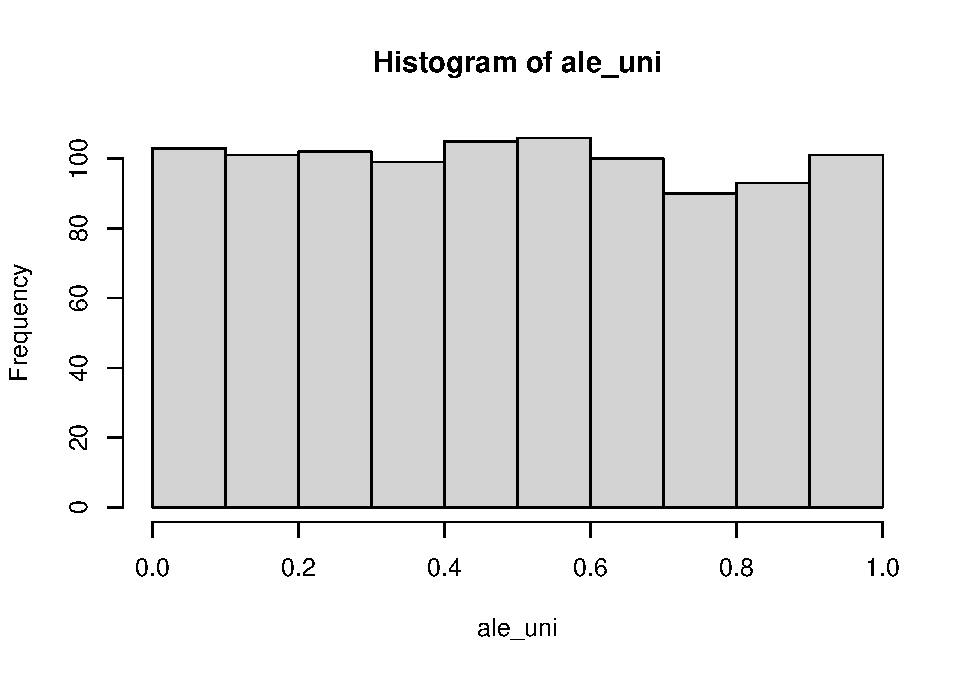
\includegraphics{Teoria4_files/figure-latex/Ejemplo distribucion uniforme-3.pdf}

\end{document}
